% This section presents the preliminary tag-week (two-way DID) results
% and the user-group/GitHub extensions that motivated the
% triple-difference design developed in detail in
% Section~\ref{sec:results}.

\subsection{Preliminary tag-week (two-way) evidence}

A useful starting point is the descriptive time series displayed in
Figure~\ref{fig:so_time_series}. Aggregate weekly questions on the
top-100 tags fell from approximately 50{,}000 in early 2020 to under
10{,}000 by late 2024. The decline accelerates noticeably around the
release of ChatGPT in November 2022, although the trajectory is
visibly downward-trending before that date as well. This descriptive
pattern motivates the need for both pre-trend-aware identification
and a within-tag, within-question-type decomposition.

\begin{figure}[!htbp]
\centering
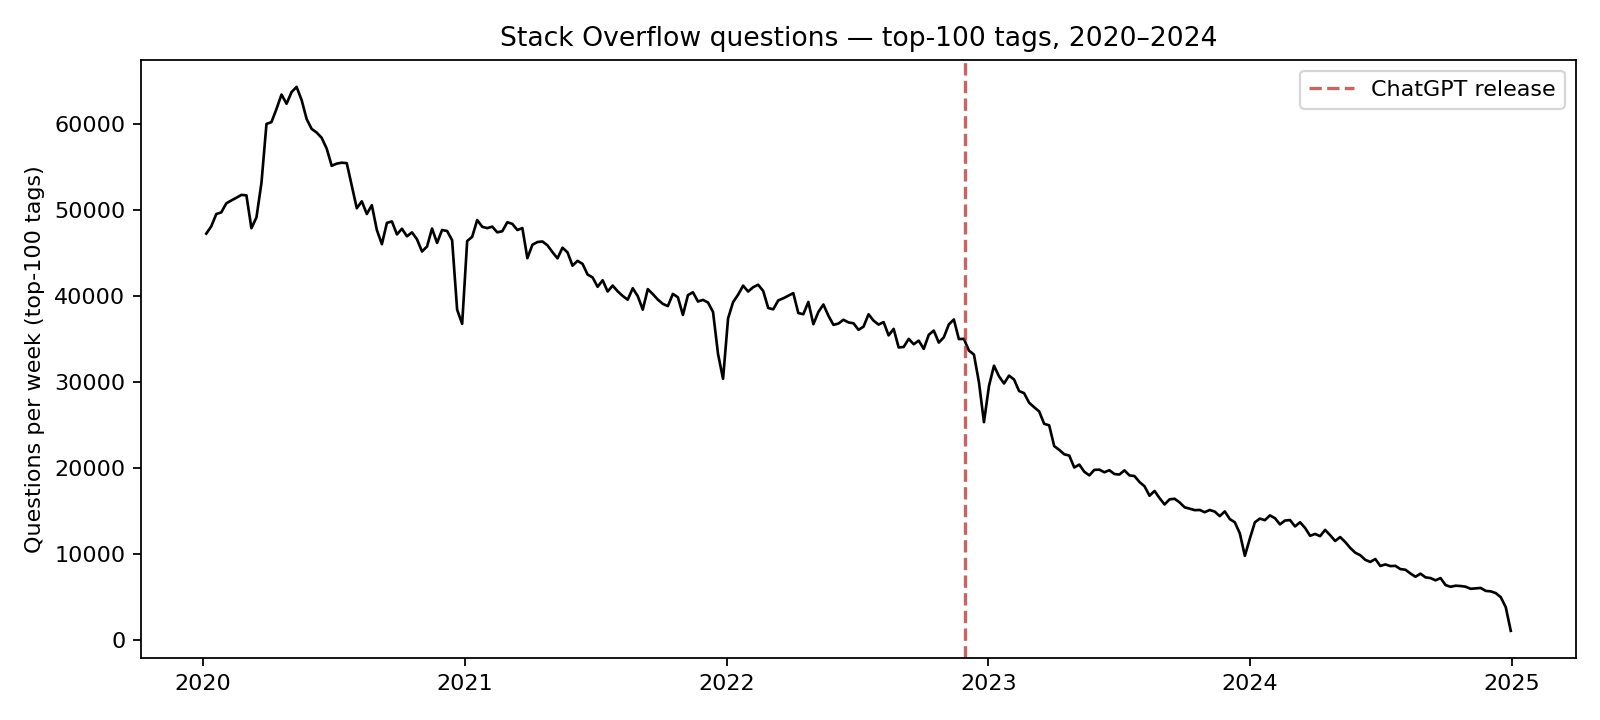
\includegraphics[width=0.95\textwidth]{figures/macro_total_weekly.png}
\caption{Total weekly Stack Overflow questions on the top-100 tags,
2020--2024. Vertical dashed line: ChatGPT public release.}
\label{fig:so_time_series}
\end{figure}

The tag-week two-way DID of Equation~\eqref{eq:did} produces the
expected sign: tags with higher pre-treatment AI answerability
declined more in questions, answers, and accepted-answer rates after
ChatGPT. The aggregated estimates (using the first-pass
\texttt{stackoverflow\_real\_results.py} pipeline) are reported in
Table~\ref{tab:integrated_results} for log questions, log answers,
accepted-answer share, and code share. We retain them here for
backward compatibility with earlier drafts, but emphasize that the
\emph{main quasi-causal claim} of the paper is now grounded in the
triple-difference design developed in Section~\ref{sec:results},
which controls for tag $\times$ question-type fixed effects and
estimates the AI-substitutability slice specifically.

\subsection{Event-study diagnostics}

The two-way DID event-study (Equation~\eqref{eq:event} but with
$\text{Sub}_k$ dropped, so only the AI $\times$ time interaction is
estimated) reveals visible pre-trends---negative coefficients in
quarters before ChatGPT---that complicate a strict
parallel-trends reading. Figure~\ref{fig:so_event_study} reports
these dynamic coefficients on log questions. The post-period
movements are substantially larger than the pre-period ones, but
the residual pre-pattern is not zero. This finding is the
motivation for moving to the triple-difference design, which
sweeps out tag-level differential trends through the
$\alpha_{t,k}$ fixed effect and estimates the within-tag
substitutable-vs-non-substitutable margin.

\begin{figure}[!htbp]
\centering
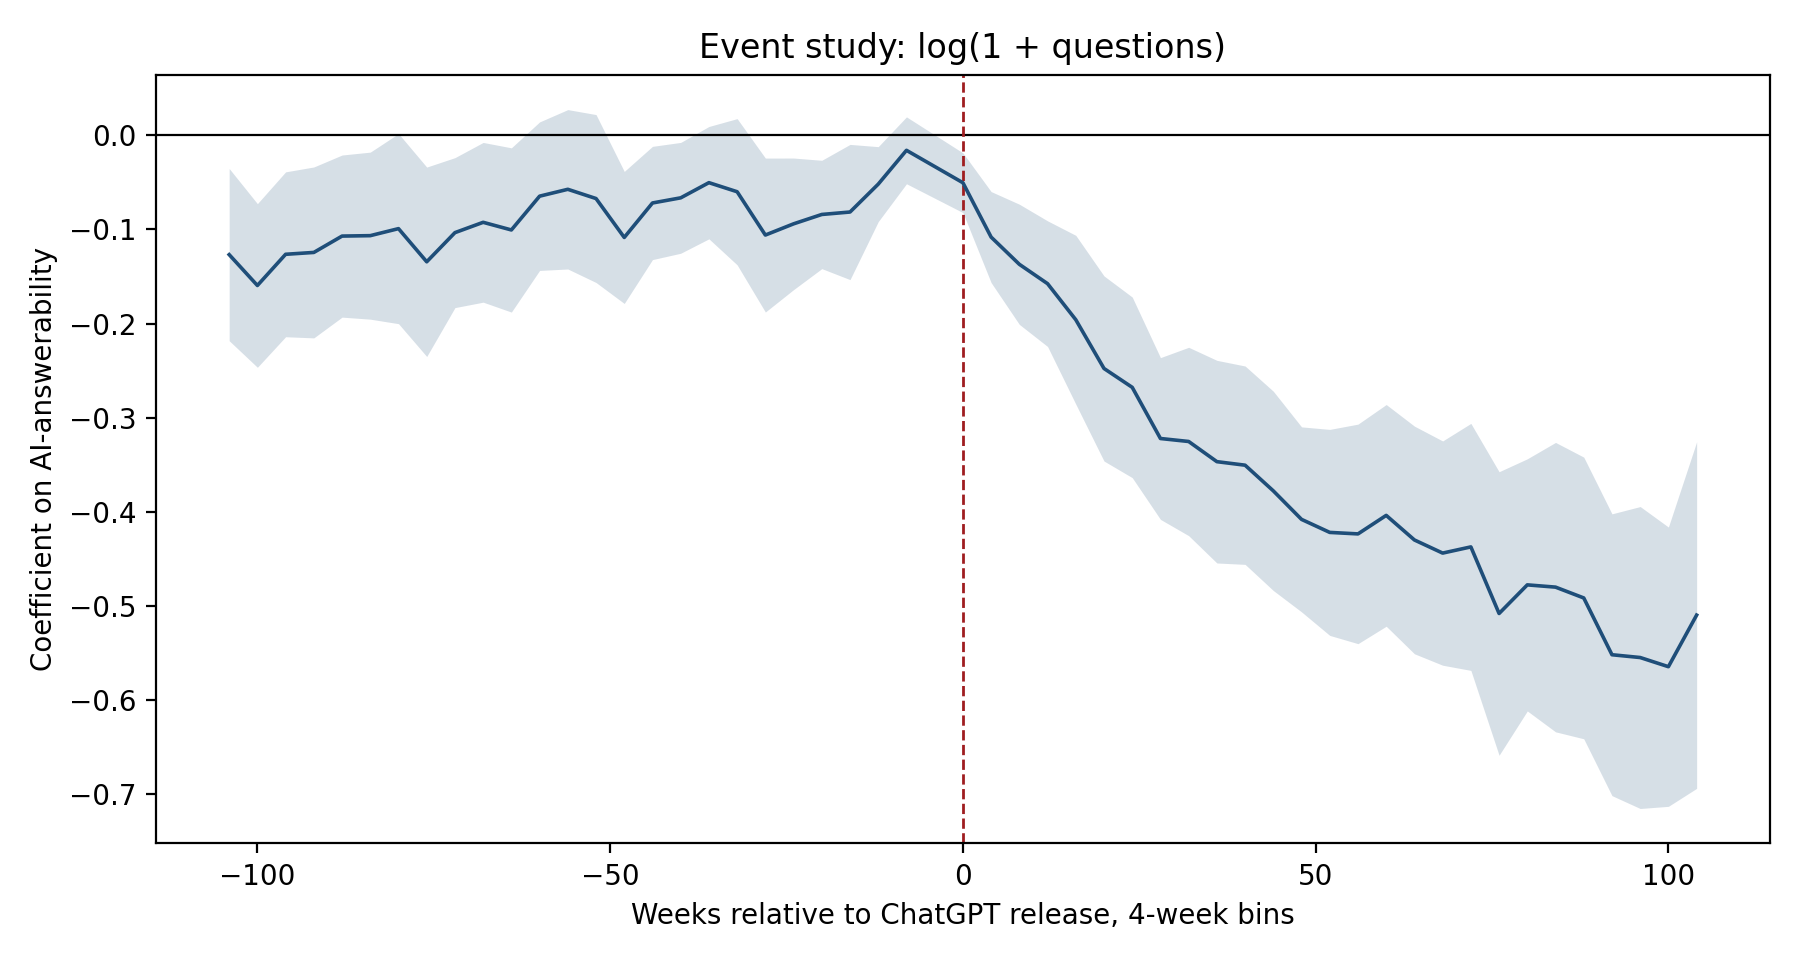
\includegraphics[width=0.95\textwidth]{figures/stackoverflow_event_study_log_questions_real.png}
\caption{Two-way DID event-study estimates for log questions
(retained from the first-pass design).}
\label{fig:so_event_study}
\end{figure}

\subsection{Secondary extensions}

The user-group panel produces estimates that are directionally
consistent with stronger declines among new and low-reputation users
in high-AI tags, but the current grouped extract is too coarse to
deliver precise differential new-user estimates. We treat the
user-entry channel as suggestive.

The GitHub extension, built from the entry-oriented GH Archive
sample (PullRequest, Issues, IssueComment, Fork, Watch events) and
public repository language metadata, does not yet show a robust
post-ChatGPT decline in entry for languages historically more
dependent on Stack Overflow. Figure~\ref{fig:github_first_seen}
plots the first-seen actors by language in the entry-oriented
sample. We retain these estimates as a bounded extension, but they
do not support a stronger downstream claim and are reported
in the Online Appendix.

% [figure moved to Online Appendix: fig:github_first_seen]

\begin{table}[!htbp]
\centering
\caption{Integrated first-pass results}
\label{tab:integrated_results}
\resizebox{\textwidth}{!}{%
\begin{tabular}{llllr}
\toprule
Block & Hyp. & Outcome & Coefficient & Estimate \\
\midrule
Stack Overflow core & H1 & SO: log(1 + questions) & AI answerability x Post ChatGPT & -0.301*** (0.070) \\
Stack Overflow core & H1 & SO: log(1 + answers) & AI answerability x Post ChatGPT & -0.254*** (0.066) \\
Stack Overflow core & H1/H3 & SO: answer rate & AI answerability x Post ChatGPT & 0.021*** (0.008) \\
Stack Overflow core & H3 & SO: code share & AI answerability x Post ChatGPT & -0.023*** (0.005) \\
Stack Overflow core & H2/H3 & SO: short-code share & AI answerability x Post ChatGPT & -0.034*** (0.005) \\
Stack Overflow trend-robust & H1 & SO: log(1 + questions) & AI answerability x Post ChatGPT & -0.331*** (0.060) \\
Stack Overflow trend-robust & H1 & SO: log(1 + answers) & AI answerability x Post ChatGPT & -0.327*** (0.053) \\
Stack Overflow user heterogeneity & H1/H2 & SO: log(1 + questions) & AI answerability x Post ChatGPT & -0.173*** (0.054) \\
Stack Overflow user heterogeneity & H2 & SO: log(1 + questions) & AI answerability x Post ChatGPT x new user & -0.089 (0.086) \\
Stack Overflow user heterogeneity & H1/H2 & SO users: log(1 + unique users) & AI answerability x Post ChatGPT & -0.149*** (0.049) \\
Stack Overflow user heterogeneity & H2 & SO users: log(1 + unique users) & AI answerability x Post ChatGPT x new user & -0.081 (0.077) \\
GitHub extension & H4 & GitHub: log(1 + first-seen actors) & SO dependence x Post ChatGPT & 0.042 (0.052) \\
GitHub extension & H4 & GitHub: log(1 + first-seen PR actors) & SO dependence x Post ChatGPT & 0.051* (0.030) \\
GitHub extension & H4 & GitHub: log(1 + first-seen issue actors) & SO dependence x Post ChatGPT & 0.014 (0.052) \\
\bottomrule
\end{tabular}
}
\begin{minipage}{0.96\linewidth}
\footnotesize
Notes: Stars denote p $<$ 0.10, p $<$ 0.05, and p $<$ 0.01. All tables are generated from reproducible scripts. GitHub estimates are exploratory because language-level inference has few clusters.
\end{minipage}
\end{table}

